\documentclass{report}

\usepackage[utf8]{inputenc}
\usepackage[T1]{fontenc}

\usepackage{graphicx}
\usepackage{float}
\usepackage{listings}
\usepackage{color}
\usepackage{hyperref}
\usepackage{datetime}
\usepackage{mathtools}

% Config taken from http://tex.stackexchange.com/a/68092
\lstset{language=C++,
  basicstyle=\ttfamily,
  keywordstyle=\color{blue}\ttfamily,
  stringstyle=\color{red}\ttfamily,
  commentstyle=\color{green}\ttfamily,
  morecomment=[l][\color{magenta}]{\#}
}

\title{\textsc{libdepixelize algorithmic documentation}}
\author{Vinícius dos Santos Oliveira}
\date{\today}

\begin{document}

\maketitle
\tableofcontents
\pagebreak

\chapter{Preface}

This document is a project to centralize the knowledge required to implement the
\href{http://research.microsoft.com/en-us/um/people/kopf/pixelart/}{Kopf-Lischinski}
vectorizer algorithm. It was created as part of the
\href{http://www.google-melange.com/gsoc/project/google/gsoc2013/vinipsmaker/48002}{GSoC
2013's libdepixelize project}.

Another goal of this document is to ease the comprehension of
\href{https://launchpad.net/libdepixelize}{libdepixelize}'s source code. That
said, documentation of techniques used in libdepixelize will be favored over
other techniques. Keep in mind that this document is \textbf{not}
documentation for the libdepixelize source code and may be useful independently
from it, but libdepixelize maintainers will greatly benefit from this document.

The initial content of this document was adapted from posts published during the
development of libdepixelize on
\href{http://vinipsmaker.wordpress.com/category/computacao/gsoc2013-inkscape/}{Vinipsmaker
labs}, the original libdepixelize author's blog. The adaptation includes:

\begin{itemize}
\item Replacing several of the media assets by higher quality files.
\item Restructure the order of the posts to make the documentation more didatic.
\item Review the text and update it to refer to the libdepixelize's current
  techniques.
\end{itemize}

All images in this document, unless explicitly stated otherwise, were created
using Inkscape and its awesome alignment tools.

This document is dedicated to the Inkscape community.

\chapter{Introduction}

Playing video games is a part of the life of several people already and in the
beginning of this new kind of entertainment, a lot of love was invested in the
creation of beautiful images where the pixels were carefully put together.

Time went by on and the age of ``pixel art'' was momentarily\ldots{}
forgotten\ldots{} replaced by more demanding art after more and more powerful
devices started to appear.

Some people were never able to forget pixel art and continued to play ancient
games just for the sake of nostalgia. The emulation community was born with the
intent to revive the classic moments and it produced some awesome tools over the
time.

In 2011, a new technology excited the emulation forums. This new technology was
an algorithm created by Johannes Kopf and Dani Lischinski that could create
resolution independent vector graphics representations out of pixel art images.

And then you came here and have this document that will surely be your lovable
guide in the challenging quest of implementing the wonderful Kopf-Lischinski
algorithm. What are you waiting for? Go on and proceed to the next page.

\section{Requirements}

Understanding Bézier curves is a must for this document and if the reader is not
very familiar with these curves, \emph{vinipsmaker} suggests you to read the
excellent \href{http://pomax.github.io/bezierinfo/}{Pomax's \emph{A Primer on
Bezier Curves}}. If you think Pomax's text is too advanced, you can start with
\href{http://jeremykun.com/2013/05/11/bezier-curves-and-picasso/}{Math $\cap$
Programming} blog.

\chapter{Splines extraction on Kopf-Lischinski algorithm}

Well, one of the phases in the algorithm is splines extraction. This phase
creates a pipeline (output from one step is the input of the next) like the
following:

\begin{enumerate}
\item It takes the color similarity graph
\item It generates a generalized Voronoi diagram
\item It groups the voronoi cells to identify visible edges
\item It generates the splines
\end{enumerate}

\hyperref[blogpart0]{Part 0} explains a fast method to compute the Voronoi
diagram exploring special properties of the input graph.
\hyperref[blogpart1]{Part 1} explains a fast method to add polygons together
exploring special properties of the generated Voronoi diagram and the data
layout used in libdepixelize. \hyperref[blogpart2]{Part 2} explains how to
generate the Bézier curves. \hyperref[tjunction]{T-junction} section discusses
how to handle T-junction nodes.

The names of the sections are based on the titles of the original posts where
they came from.

\section{Part 0}
\label{blogpart0}
Originally posted at
\url{http://vinipsmaker.wordpress.com/2013/07/22/splines-extraction-on-kopf-lischinski-algorithm-part-0/}
on \formatdate{22}{7}{2013}.

\subsection{Generalized Voronoi diagram generation}

Well, a Voronoi diagram is a black box where you put some points (the seeds) and
you get some polygons (the cells). Each polygon contains all points that are
closer to its seed than any other seed. There is a
\href{http://en.wikipedia.org/wiki/Voronoi_diagram}{good article on Wikipedia}
and I won't explain any further.

Kopf-Lischinski algorithm executes a bunch of operations on a graph and it uses
a Voronoi diagram to extract a visual representation from this graph. The
simplest form of a Voronoi diagram works with 2D points-seeds, but we have
higher-dimentional Voronoi diagrams, Voronoi diagrams using different distance
functions and even Voronoi diagrams using complex non-points seeds. We are
interested in these Voronoi diagrams using complex non-points seeds.

The below image has a representation of the output graph of the Kopf-Lischinski
algorithm and its Voronoi diagram representation. The graph nodes are
represented by circles, where nodes with the same color are similar and usually
are connected. The connections of the nodes are represented by green lines.

\begin{figure}[H]
  \centering
  \includegraphics[width=0.8\textwidth]{assets/accurate_voronoi.pdf}
  \caption{An accurate generalized Voronoi diagram}
\end{figure}

The generalized Voronoi diagram is visual --- there is no special meaning to
explain it in the previous image. The seeds of this diagram aren't points, they
are line segments. You just need to break a green line in two and add each half
to its containing cell. You can note that some polygons aren't
\href{http://en.wikipedia.org/wiki/Convex_polygon}{convex}.

The graph used as input has certain constraints that enable us to use some
simple and fast operations instead of a
\href{http://en.wikipedia.org/wiki/Fortune\%27s_algorithm}{full-featured and
complex algorithm}.

If a Voronoi cell is a polygon containing all points that are closer to its seed
than any other seed, we can determine the edge of a Voronoi cell by the midpoint
of two adjacent seeds. If we generate a vertex for each of its 8 directions, we
will get an accurate Voronoi diagram.

\begin{figure}[H]
  \centering
  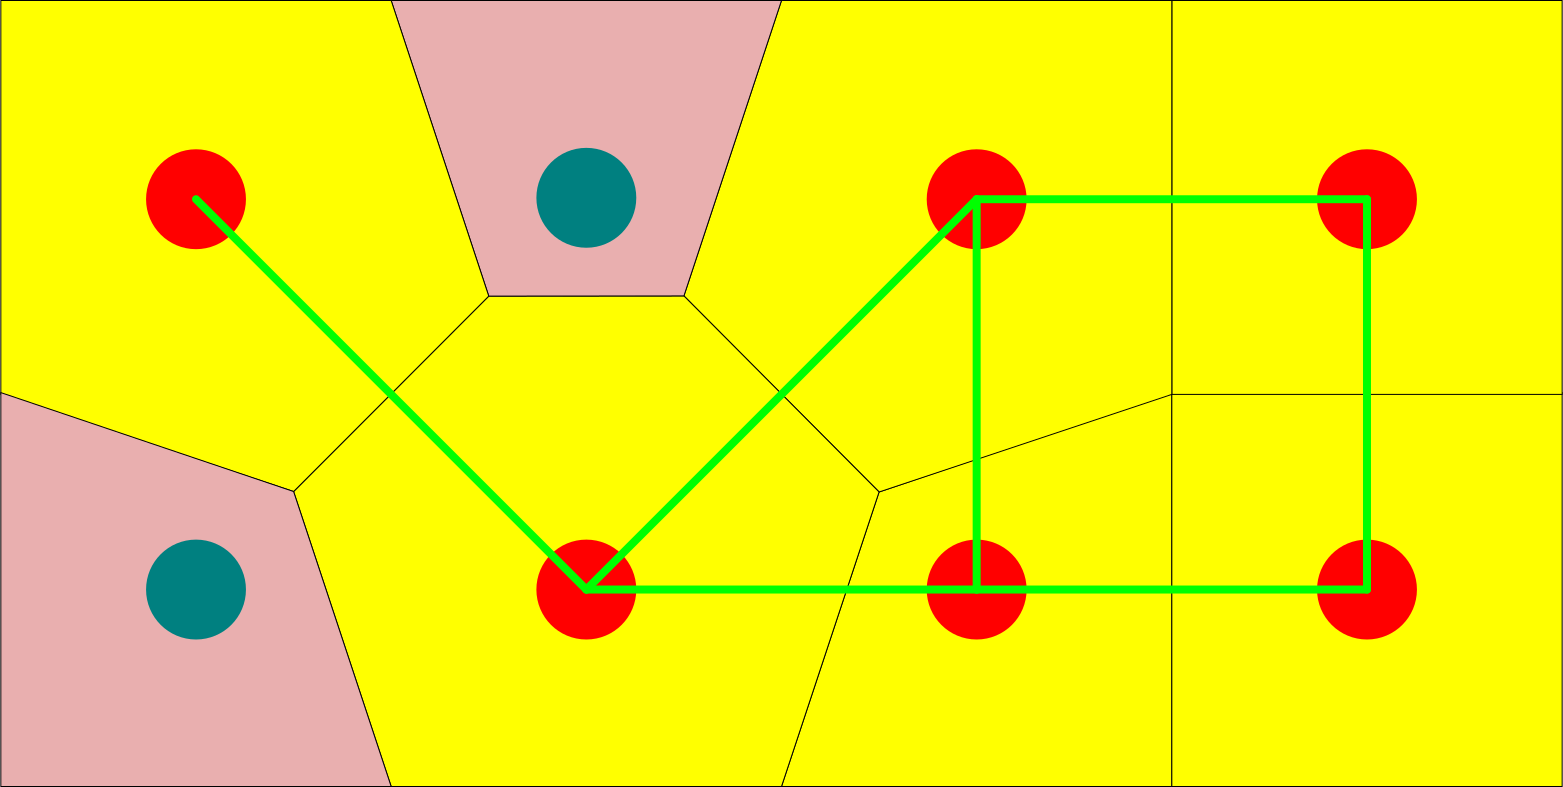
\includegraphics[width=0.8\textwidth]{assets/voronoi.pdf}
  \caption{A simplified generalized Voronoi diagram}
\end{figure}

We can get a simplified Voronoi diagram by forgetting about the top, bottom,
left and right vertices (if we just generate the diagonal vertices). The
simplified version doesn't contain
\href{http://en.wikipedia.org/wiki/Concave_polygon}{concave polygons}.

The act of generating diagonal vertices is more complex than the act of
generating the other vertices. We need to check if there is a connection with
the other cell and, if this connection exists, generate two vertices. If the
connection doesn't exist, we generate a single vertex, but its position depends
on the existence of a connection between its neighbors. Look the following
figure.

\begin{figure}[H]
  \centering
  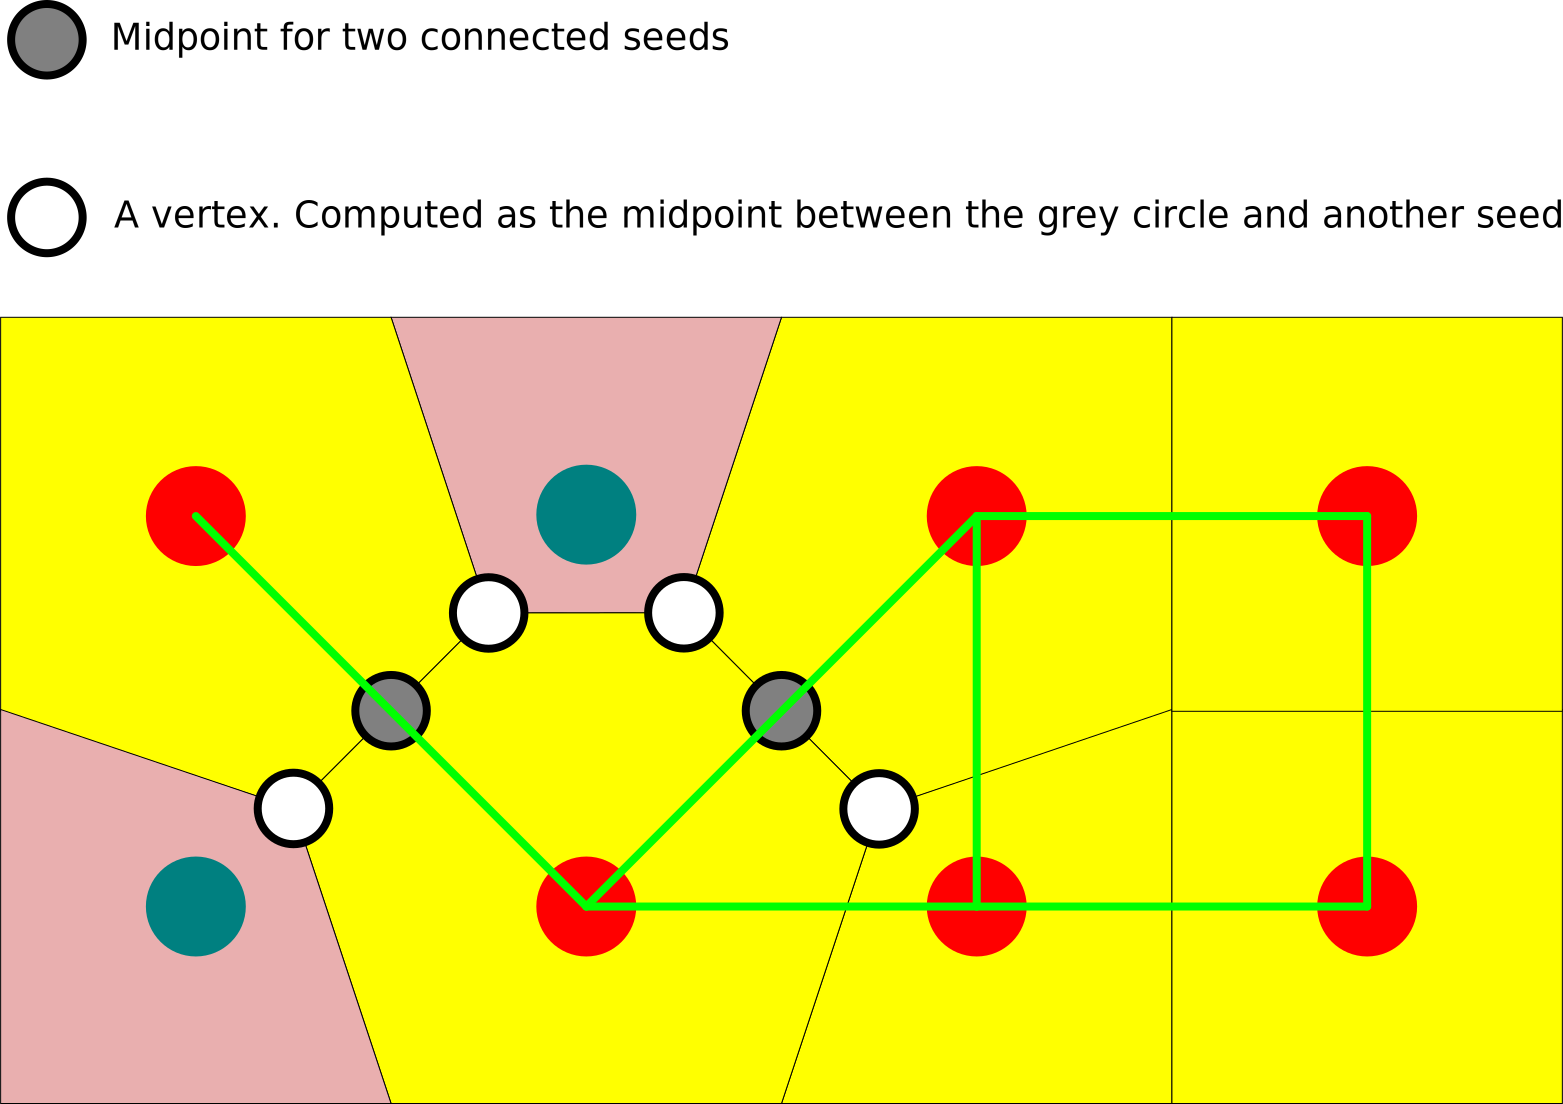
\includegraphics[width=0.8\textwidth]{assets/voronoi2.pdf}
  \caption{A simplified generalized Voronoi diagram (detailed)}
\end{figure}

All information we need to generate the Voronoi diagram is located within its
neighbors and the only extra tool we need to generate the points is the midpoint
procedure.

\subsection{Metadata extraction}

When we generate B-Splines using Kopf-Lischinski algorithm we need a way to
separate points that create sharp corners and smooth points. The Kopf-Lischinski
algorithm has techniques just to handle this issue. In libdepixelize, the point
smoothness computation and Voronoi generation are merged in one single phase.
This is the phase where we can gather lot of info about the graph and we can
propagate the smoothness data to later phases.

One note about the algorithm of this ``metadata extraction'' section is that
some points will disappear during polygon union and we don't care if the
metadata about these points is accurate, then we can simplify the algorithm
exploring this property.

Unfortunately (for the implementer only), graph nodes of different colors can be
grouped and if we don't intend to discard this \emph{extra color information}
(an extension of Kopf-Lischinski on its own), a special care must be taken to
handle these nodes. libdepixelize has some extensions that are documented later
in this document. But for now, to ease explanation, we consider only cells of
equal colors can be connected.

The below image has some features that will be citated in this subsection to
explain how the algorithm works:

\begin{figure}[H]
  \centering
  \includegraphics[width=0.8\textwidth]{assets/voronoi3.pdf}
  \caption{Vertex types}
\end{figure}

There are two types of vertices generated in this special Voronoi diagram:

\begin{itemize}
\item White type: The type of the one labelled with ``\#1''. Node ``\#1'' is
  contained by three cells, one purple and two yellows. The two yellow cells
  will be merged during polygon-union. There are two possibilities for the
  remaining cell in this kind of node:
  \begin{itemize}
  \item When it has the same color. Then the node will disappear during
    polygon-union and we don't care about its \emph{smoothness} attribute.
  \item When it has a different color. Then we say it is a valence-2 node.
  \end{itemize}
\item Cyan type: The type of the one labelled with ``\#2''. This type of node can
  appear in the border of the image and isn't smooth or in the center of 4 cells
  and its smoothness isn't predictable in advance. If it appears in the center
  of four cells, then:
  \begin{itemize}
  \item It can be in the middle of 4-connected cells and we don't care about its
    \emph{smoothness} attribute, because this node will disappear.
  \item It can be in the middle of a valence-2 node and will be smooth.
  \item It can be a valence-3 node and things start to get complex. After the
    polygon union, this node will be part of three different polygon and only
    two of these three nodes will share the same value for the \emph{smoothness}
    attribute.
  \end{itemize}
\end{itemize}

With these problems explained, it's time for the algorithm! The algorithm is
kind of repetitive (if we iterate the bottom-right node, compare with bottom and
right cells, then do all it again, but use nodes of different
directions\ldots{}), but the principle is the same for all ``repetitive'' code,
then only the important parts are documented here. If you really want to see the
whole thing, see appendix \ref{smoothness_code_appendix}.

\begin{figure}[H]
  \centering
  
\includegraphics[width=0.8\textwidth]{assets/layout.pdf}
\end{figure}

The above image represents the analysed data in the following code example,
except for the fact that we don't know what are the colors of the cells. We are
iterating on the middle point of the image and the current iterated cell is cell
A. The algorithm also uses the concept of \emph{shading edge} and \emph{contour
edge} described in Kopf-Lischinski paper.

\lstinputlisting[language=C++,frame=single]{assets/code/smoothness.cpp}


\section{Part 1}
\label{blogpart1}
Originally posted at
\url{http://vinipsmaker.wordpress.com/2013/07/21/splines-extraction-on-kopf-lischinski-algorithm-part-1/}
on \formatdate{21}{7}{2013}.

\subsection{Polygon union}

Polygons can be represented by vertice points. libdepixelize stores them in
clockwise order, with the first point being part of the polygon's
northwest/top-left. One important feature of the generated Voronoi diagram
is that all ``connected'' cells share a common edge.

The algorithm can be described in 4 major steps:

\begin{enumerate}
\item Find the largest common edge
\item Remove the in-between points of the common edge
\item Choose one polygon and refer to it as P (choose the smallest polygon for
  better performance)
  \begin{enumerate}
  \item 
    Shift P such as P's head and tail are points of the common edge
  \end{enumerate}
\item Choose the other and refer to it as Q
  \begin{enumerate}
  \item Remove one of the common edge's points in Q
  \item Replace the remaining point that is part of the common edge in Q by P's
    points
  \end{enumerate}
\end{enumerate}

The Voronoi cells are iterated one by one, line by line, from the left-most cell
to the right-most cell. This behaviour could change in favor of a
\href{http://en.wikipedia.org/wiki/Cache-oblivious_algorithm}{cache-oblivious
algorithm}.

We check if (1) we already have a group of the current color, (2) the existing
group has a common edge with current Voronoi cell and, then, (3) we add the
current Voronoi cell to the existing polygon. Beware that the Voronoi cells from
the input are always convex polygons, but the existing polygon (that groups the
Voronoi cells) might be
\href{http://en.wikipedia.org/wiki/Concave_polygon}{concave}.

Let's see an example of the algorithm. In the example, we are iterating in the
second line and we found an existing grouping polygon with a matching color (the
two entities are connected), then we must add them togheter. The image below
represents the situation we are interested in:

\begin{figure}[H]
  \centering
  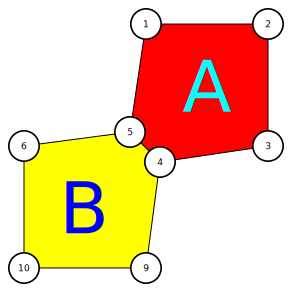
\includegraphics[width=0.8\textwidth]{assets/polygon-union.pdf}
\end{figure}

Polygon A is represented by the list of points [1, 2, 3, \textbf{4}, \textbf{5}]
(common edge's points in bold). Polygon B is represented by the list of points
[6, \textbf{7}, \textbf{8}, 9, 10] (common edge's points in bold). Points 4 and
8 are equal and points 5 and 7 are equal. Polygon A is the grouping polygon
while polygon B is the current Voronoi cell. We shift B's list to [\textbf{8},
9, 10, 6, \textbf{7}] and use it to get the final polygon [1, 2, 3, 8, 9, 10, 6,
7].

Let's do it one more time:

\begin{figure}[H]
  \centering
  \includegraphics[width=0.8\textwidth]{assets/polygon-union2.pdf}
\end{figure}

Polygon A is the grouping polygon, represented by [1, 2, \textbf{3}, \textbf{8},
\textbf{9}, 10, 6, 7]. Polygon C is the current Voronoi cell and is represented
by [\textbf{11}, \textbf{12}, 13, \textbf{14}]. This time the largest common
edge have 3 points and point 8/11 is the in-between point, then we remove it.
The resulting A polygon is [1, 2, \textbf{3}, \textbf{9}, 10, 6, 7] and the
resulting C polygon is [\textbf{12}, 13, \textbf{14}]. When we replace the
common edge interval in A by C, we get the final polygon, [1, 2, \textbf{12},
13, \textbf{14}, 10, 6, 7]. The final polygon is show in the image below:

\begin{figure}[H]
  \centering
  \includegraphics[width=0.8\textwidth]{assets/polygon-union3.pdf}
\end{figure}

One last note that might be useful in later steps is the access pattern used by
the algorithm. When we add a voronoi cell to the grouping polygon, there is a
hot area and a cold area. The cold area is the area where there will never be a
common edge. These areas always are concetrated in the same places, like
exemplified by the following image:

\begin{figure}[H]
  \centering
  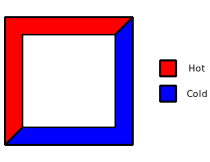
\includegraphics[width=0.8\textwidth]{assets/hot-cold.pdf}
\end{figure}

\subsection{Splines generation}

The previous step look simple, but there may be additional info that we may want to
store for each node. This (polygon-union) is the last step where we still can
gather locality info without executing a deep lookup.

\begin{figure}[H]
  \centering
  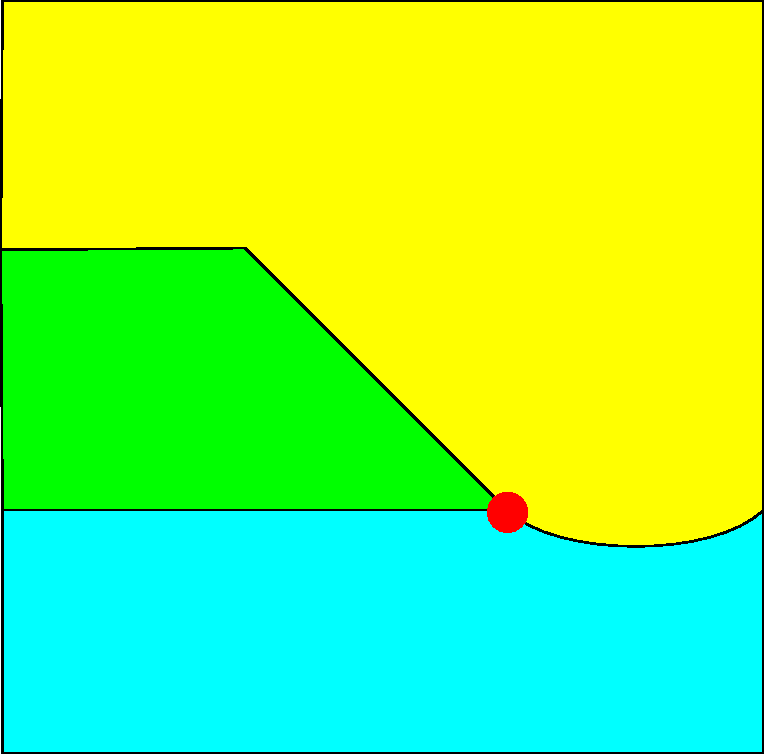
\includegraphics[width=0.8\textwidth]{assets/valence-3-node.pdf}
  \caption{Valence-3 node (in red)}
\end{figure}

Let's refer to nodes where at most two different grouping polygons share a point
as valence-2 nodes. There are valence-2 nodes, valence-3 nodes and valence-4
nodes. Valence-2 nodes are always smooth and valence-4 nodes never are smooth,
but valence-3 nodes vary.

\begin{figure}[H]
  \centering
  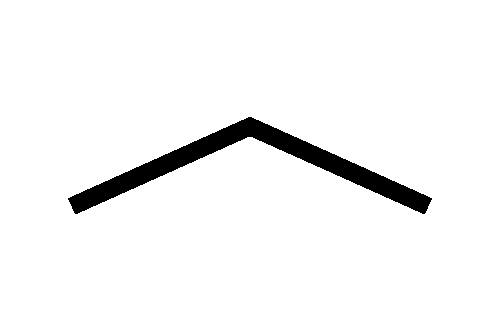
\includegraphics[width=0.8\textwidth]{assets/non-smooth.pdf}
  \caption{Non-smooth node}
\end{figure}

Most of the points are shared by nodes of different polygons and when we have
three valence-3 nodes, exactly only one of them will be smooth. We apply
Kopf-Lischinski algorithm heuristics to determine which one will be and store
this info for later usage.

\begin{figure}[H]
  \centering
  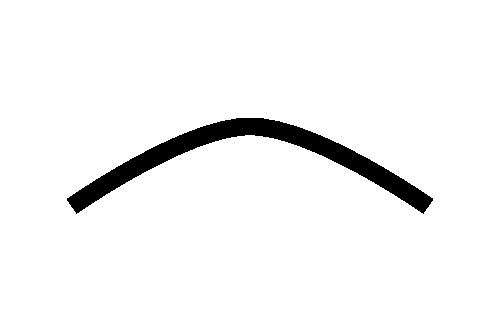
\includegraphics[width=0.8\textwidth]{assets/smooth.pdf}
  \caption{Smooth node}
\end{figure}

The complicated part about the splines extraction on Kopf-Lischinski algorithm
is the overlapping between these last steps (group the Voronoi cells to identify
visible edges and generate the splines).

\subsection{A bit of performance}

So, Kopf-Lischinski algorithm resembles a compiler. You have several data
representation types and each type offers different operations. You explore the
operations each type offers and convert it to another representation until you
reach the final result. In several of the type representations used by the
Kopf-Lischinski algorithm, you have a matrix and you access each element and its
neighbours.

\begin{figure}[H]
  \centering
  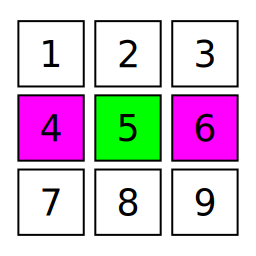
\includegraphics[width=0.8\textwidth]{assets/memory-access.pdf}
  \caption{Access pattern representation}
\end{figure}

The particular implementation for libdepixelize stores and access the elements
linearly like [1, 2, 3, 4, 5, 6, 7, 8, 9]. It could make good use of processor
cache, but ain't that easy. Suppose we are iterating on element 5, then we need
to access all its neighbours, but only neighbours 4 and 6 may be in cache,
especially in large images. This is the first problem in cache usage of the
implementation, but we cannot remove this usage pattern, because it's part of
the algorithm and there is a data dependency among the elements. However, we can
change the memory layout to favor the usage pattern. This technique is called
\href{http://en.wikipedia.org/wiki/Cache-oblivious_algorithm}{cache-oblivious
algorithm} and future versions of libdepixelize might implement it.

Another problem with the current data access pattern is that each element store
a complex object that may point to other regions of memory and add a level of
indirection that can contribute to cache miss. One idea that can increase the
cache hit is the one behind the
\href{http://stackoverflow.com/questions/10315041/meaning-of-acronym-sso-in-the-context-of-stdstring}{Small
String Optimization}. This change would highly increase data locality and fits
well in Kopf-Lischinski algorithm, because the complex objects stored by each
element in every phase tends to have a small maximum number of subelements.


\section{Part 2}
\label{blogpart2}
Originally posted at
\url{http://vinipsmaker.wordpress.com/2013/08/13/splines-extraction-on-kopf-lischinski-algorithm-part-2/}
on \formatdate{13}{8}{2013}.

\subsection{Once upon a time\ldots{} a polygon with holes appeared}

The polygon-union described in \hyperref[blogpart1]{part 1} works correctly and
there are no better answers than the correct answer, but these polygons were
meant to be B-Splines and what have been done till now is insufficient.

Consider the following image.

\begin{figure}[H]
  \centering
  
\includegraphics[width=0.8\textwidth]{assets/polygon-holes.pdf}
  \caption{Normal polygon (left) and bordered polygon (right)}
\end{figure}

The left polygon is the polygon what you see before and after the polygon-union.
They are visually indistinguishable. The right polygon has an outline to allow
you understand its internal representation. You can understand how the
polygon-union generates a polygon with a ``hole'' seeing the right polygon.

If the polygon-union don't generate visually identifiable pixels, then there
shouldn't exist any problem, but when we convert the polygon to a B-Spline, some
areas of the image won't be filled. The polygons won't fit correctly, like show
in the image below.

\begin{figure}[H]
  \centering
  
\includegraphics[width=0.8\textwidth]{assets/polygons-with-holes-and-splines.pdf}
  \caption{After B-Spline conversion}
\end{figure}

The solution is to create some holes. With the representation of polygons used
in libdepixelize, this task is very simple and the key operation to accomplish
this goal is to find the ``edges that the polygon share with itself''. The
following paragraphs explain this task.

\begin{figure}[H]
  \centering
  
\includegraphics[width=0.8\textwidth]{assets/polygon-holes-conversion.pdf}
\end{figure}

The above image has 2 pairs of hidden points: pair <5, 6>, that is equal to pair
<11, 10>, and pair <12, 13>, that is equal to pair <18, 17>.


The algorithm outline is:

\begin{enumerate}
\item Iterate over the points and, for each point, try to find another point
  that is equal to it. For each point
  \begin{enumerate}
  \item Get the internal sequence. To gather the internal sequence, just iterate
    over more nodes to get the ``largest common edge''.
  \item Make sure the ``largest common edge'' has a size greater than 1 (e.g. is
    not only a common vertex, but a common edge). Use this sequence to construct
    the internal ``hole'' (or holes, if more than one) polygon and then remove
    it from the original polygon.
  \end{enumerate}
\end{enumerate}

Beware that \emph{use a sequence to construct the internal ``hole'' polygon} is
another algorithm (and ain't trivial). It goes like this (let's name it
\emph{fill\_holes}):

\begin{enumerate}
\item Create an empty sequence of nodes. Let's name it \emph{hole}.
\item Let's name the beginning of our input sequence \emph{region\_begin}.
\item Iterate over the nodes of sequence and for each node:
  \begin{enumerate}
  \item Find another node equal to this one and if there is such node:
    \begin{enumerate}
    \item Let's name our new finding \emph{aux}.
    \item Append a copy of the range from \emph{region\_begin} until the current
      node (do \textbf{not} confuse the current node with \emph{aux}) into
      \emph{hole}
    \item We can see a common vertex: Current node and \emph{aux}. Find the
      largest common edge and there will be references to two more nodes. Call
      \emph{fill\_holes} with this new range.
    \item Forget about the range between current node and \emph{aux}. We won't
      see these points in the next iteration and \emph{region\_begin} will refer
      to \emph{aux} from now on.
    \end{enumerate}
  \end{enumerate}
\item Append the range from \emph{region\_begin} until the end of input
  sequence into \emph{hole}.
\item \emph{hole} is ready. Do something with it (e.g. store it).
\end{enumerate}

The \emph{fill\_holes} procedure is complicated and you should check
libdepixelize's source code (\emph{HomogeneousSplines::\_fill\_holes}) to kill
any ambiguity or doubt.

\begin{itemize}
\item Remark \#1: libdepixelize do the steps of the outmost algorithm (the one
  removing nodes from the sequence) in backward order, to avoid too much moves
  of elements in the internal vector.
\item Remark \#2: The polygon is represented in clockwise order, but the holes
  will be represented in counter-clockwise order, but there is no reason to
  normalize. You can safely ignore this (de)normalization feature.
\item Remark \#3: The reason behind the special procedure to make sure the
  common sequence is an edge and not a vertex come from the fact that the code
  to fix the position of   T-junction nodes creates a pattern where the polygon
  shares a point with itself.
\end{itemize}

\subsection{And then, the polygon was meant to be a B-Spline}

It's a chapter about splines extraction and it's fair to end with this step.

\begin{figure}[H]
  \centering
  
\includegraphics[width=0.8\textwidth]{assets/evolution.pdf}
  \caption{It's evolution, baby}
\end{figure}

The algorithm is very simple. The points you get through the polygon-union
algorithm in \hyperref[blogpart1]{part 1} will be the control points of
quadratic Bézier curves and the interpolating/ending points of each Bézier curve
will be the middle points between two adjacent control points. This is the
special case where all points are smooth. The image below can help you get the
idea.

\begin{figure}[H]
  \centering
  
\includegraphics[width=0.8\textwidth]{assets/points-location.pdf}
  \caption{Locations of the B-Spline points}
\end{figure}

If you have non-smooth points, then all you need to do is interpret them as
interpolating points, instead of control points. You'll have three interpolating
points that are part of two straight lines. There is a bit more of theory to
understand why the generated B-Spline is smooth.


\section{T-junctions}
\label{tjunction}
In this section the problem of how to adjust the endpoint of a curve to properly
lie on the other curve will be discussed.

Per Kopf-Lischinski, a T-junction node will be the node that is common for three
adjacent splines. For one of the splines, this will be a smooth node. Using the
the shading/contour edges heuristic with an unspecified input image, we get the
following output:

\begin{figure}[H]
  \centering
  
\includegraphics[width=0.8\textwidth]{assets/shading-heuristic.pdf}
  \caption{The non-blue splines share a shading edge}
\end{figure}

Some splines got visually disconnected and created an undesired result. To fix
this issue we adjust the endpoint of the non-blue curves to properly lie on the
blue curve. The end result will be the following image:

\begin{figure}[H]
  \centering
  
\includegraphics[width=0.8\textwidth]{assets/shading-heuristic-fixed.pdf}
\end{figure}

Kopf-Lischinski paper don't document extensively how to ``adjust the endpoint of
a curve to properly lie on the other curve'' and you'll need to verify that the
algorithm documented here is correct based on the sample images provided in the
paper.

You may had learnt how to generate the splines in \hyperref[blogpart2]{part 2}.
And you know that if you change the position of a node, the midpoint between
this node and adjacent nodes will change. With the midpoint being changed, the
parts that previously were fitting together will visually disconnect or overlap.
Given that, we cannot simply adjust some node position without screwing up parts
of the curve that were previously correct using the poor and simple data
representation from the other steps.

We don't want to change the representation too, because this is exactly the type
of representation expected by the optimizer in the next steps. We can, however,
insert extra nodes without screwing up the previously correct parts of the curve
and if we take care to make some of them collinear, then they won't interfere
with the visual representation we got.

Combining the previous idea with the idea of subdivision from
\href{http://en.wikipedia.org/wiki/De_Casteljau's_algorithm}{De Casteljau's
algorithm} it's possible to adjust the ``endpoint'' of the non-blue curves to
properly lie on the blue curve. It's just a matter of finding the correct
positions.

\begin{figure}[H]
  \centering
  
\includegraphics[width=0.8\textwidth]{assets/subdivision.pdf}
  \caption{\textbf{Splines} with control points highlighted with green circles}
\end{figure}

\begin{figure}[H]
  \centering
  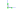
\includegraphics[width=0.8\textwidth]{assets/subdivision2.pdf}
  \caption{Blue \textbf{Bézier curve} with its points highlighted with green
    circles}
\end{figure}

After we subdivide a Bézier curve into two, there will be a new Bézier curve for
each other curve whose ``endpoint'' should properly lie on this curve. As such,
we only focus on one curve at each time. Now that we have the Bézier curve, we
need to compute the position of the new splines nodes exploring the
\emph{midpoint} feature. This process is represented in the next picture.

\begin{figure}[H]
  \centering
  
\includegraphics[width=0.8\textwidth]{assets/subdivision3.pdf}
  \caption{\textbf{Spline} with its control points highlighted with green
    circles. Yellow point is the point where the ``endpoint'' of the other
    curves should be placed.}
\end{figure}

The final result will have 5 points instead of one for a ``vertex'':

\begin{itemize}
\item The initial point to avoid screwing parts of the curve that previously
  were correct. Note that this point won't be visible, because it will be
  collinear with its neighbours points.
\item The new three points to properly adjust the ``endpoint'' of this curve.
  Note that extreme points (the first and the third) won't be visible, because
  they are collinear with its neighbour points.
\item The endpoint of the \textbf{Bézier curve}, then the two curves that are
  adjusted won't overlap. Note that this point is \textbf{not} smooth.
\end{itemize}

You may want to store this \emph{visibility} metadata for easily discard these
extra points when you convert the splines to Bézier curves in later steps.

This is the technique to ``adjust the endpoint of a curve to properly
lie on the other curve'', but this problem is not so easy, because (1) you'll
have to implement code to handle each node in the three splines and (2) the
position of nodes will also depend on the color similarity with neighbour
splines. The problem \#2 is exemplified in the image below (when compared to
previous examples):

\begin{figure}[H]
  \centering
  
\includegraphics[width=0.8\textwidth]{assets/subdivision4.pdf}
  \caption{\textbf{Splines} with its control points highlighted with green
    circles.}
\end{figure}

Usually you will have to handle four different possibilities for \textbf{each}
of the five nodes. This means four large conditional branches. Nothing pleasant,
but you can reduce the code if you find the \emph{amount} that each condition
contributes to the final result.

You can find these conditions playing with experiments and boolean algebra or,
using a more elaborate approach, solving a simple linear system. This text won't
document all possible constants (at least not for this initial release) that you
can find, but you can check libdepixelize source code if you are in such a
hurry. This text will, however, give an example of how to solve a linear system
to find such constants.

These conditions are always related to connectivy among local nodes and will be
translated in expressions like ``is node X connected to its topleft node?''.

The constants $\frac{3}{16}$, $\frac{1}{16}$ and others happen a lot in this
problem. If you know a cool name for these constants, ping \emph{vinipsmaker}
and he will be happy to use your suggestion to name these constants.

\subsection{Solving the linear system}

Suppose that you have conditions \emph{A} and \emph{B} to determine the position
of the nodes, then you have four possibilities/branches to determine the
position of the nodes.

Suppose that, for the first node, you find the following positions for the
x-axis given the input conditions:

\begin{center}
  \begin{tabular}{|c|c|r|}
    \hline
    \textbf{\emph{A}} & \textbf{\emph{B}} & position \\
    \hline
    \emph{true} & \emph{true} & 0.0625 \\
    \emph{true} & \emph{false} & 0.09375 \\
    \emph{false} & \emph{true} & 0.09375 \\
    \emph{false} & \emph{false} & 0.125 \\
    \hline
  \end{tabular}
\end{center}

Now you can convert the previous table to a linear system replacing \emph{false}
by 0, \emph{true} by 1 and adding a column completely filled with ones for the
base value. For the previous table, this procedure will generate the following
augmented matrix:

$$\left(
  \begin{array}{ccc|r}
    1 & 1 & 1 & 0.0625 \\
    1 & 0 & 1 & 0.09375 \\
    0 & 1 & 1 & 0.09375 \\
    0 & 0 & 1 & 0.125
  \end{array}
\right)$$

After solve the system, you'll get the values $-\frac{1}{32}$, $-\frac{1}{32}$
and $\frac{1}{8}$ for $\chi_1$, $\chi_2$ and $\chi_3$, respectively. $\chi_3$ is
the base value, then the equation for the x position of the first node will be:

\begin{center}
  \texttt{node.pos.x} = $\frac{1}{8} - \text{\emph{A}} \frac{1}{32}
  - \text{\emph{B}} \frac{1}{32}$
\end{center}

Because $\chi_1$ and $\chi_2$ values are equal in this particular case, we can
reduce the formula:

\begin{center}
  \texttt{node.pos.x} = $\frac{1}{8} - (\text{\emph{A}}
  + \text{\emph{B}}) \frac{1}{32}$
\end{center}

That's it! Have fun finding the constants for each $x$ and $y$ for each node for
each ``adjust the endpoint of a curve to properly lie on the other curve''
procedure.


\chapter{The \emph{extra color information} patch}
\label{extracolor}
When you apply the polygon-union algorithm from \hyperref[blogpart1]{part 1},
you face a challenging question: What should we do if we find polygons that have
similar colors and these colors are different? Kopf-Lischinski paper don't
explore this issue at all and the results from their
\href{http://research.microsoft.com/en-us/um/people/kopf/pixelart/supplementary/index.html}{supplementary
material} show random results (sometimes the color information is simply lost
and sometimes they are preserved and smoothed by the rendering technique
chosen).

libdepixelize's approach is to preserve as much color information as possible
and this approach led to some extensions to the algorithm (with more to come).
The first rule is:

\begin{equation}
  \label{ec:foundation}
  \text{\textbf{Don't discard color information\ldots ever}!}
\end{equation}

The effect of the rule \ref{ec:foundation} is that only polygons of the same
color should be united together.

But if I don't discard color information, the splines will become visually
disconnected. What should I do? First, let's review the node types with the
following image:

\begin{figure}[H]
  \centering
  \includegraphics[width=0.8\textwidth]{assets/voronoi3.pdf}
  \caption{Vertex types}
\end{figure}

There are special heuristics about what to do for each node type and these
heuristics are organized in some sections below.

Another interesting figure to introduce is the \emph{boof} character.
\emph{Boof} has a color palette and pixel patterns that help to explain the
heuristics responsible for extra color information. The Voronoi diagram
generated by boof input is shown below.

\begin{figure}[H]
  \centering
  
\includegraphics[width=0.8\textwidth]{assets/boof_voronoi.pdf}
  \caption{\emph{Boof}, kindly created by Jabiertxo Arraiza Cenoz and
    ``licensed'' under public domain (CC0).}
\end{figure}

\section{Cyan (\#2) nodes}
\label{cyan_nodes}

If you find a node for which the surrounding cells have similar colors, but not
equal, then you check if the colors of both sides of an edge are equal. There
are four edges and the node will be smooth if the total number of ``equal
colors'' counts two.

The following picture highlight the separating edges you need to check.

\begin{figure}[H]
  \centering
  
\includegraphics[width=0.8\textwidth]{assets/boof_cyan.pdf}
  \caption{Cyan node where the interesting separating edges are highlighted in
    green.}
\end{figure}

The result of this heuristic for the previous picture follows:

\begin{figure}[H]
  \centering
  
\includegraphics[width=0.8\textwidth]{assets/boof_cyan2.pdf}
  \caption{Cyan node highlighted with a green circle.}
\end{figure}

\subsection{Why does it work?}

We have a heuristic and its results are quite good, but maybe you're
wondering\ldots why does it work?

First requirement for \emph{some} of these heuristics work is:

\begin{equation}
  \label{ec:same answer}
  \text{The answer must be the same for all nodes sharing the same position.}
\end{equation}

And our heuristic fulfill the requirement \ref{ec:same answer}, because it uses
the same local data for all four nodes sharing the same position.

If a heuristic don't fulfill the requirement \ref{ec:same answer}, then it
should have extra effects such as ``adjust B-Spline'' to produce good results.

The other requirement for a good heuristic is:

\begin{equation}
  \label{ec:visually connected}
  \text{The result shouldn't create distant or overlapping segments.}
\end{equation}

And this heuristic fulfill the requirement \ref{ec:visually connected} too,
because it only creates smooth nodes when three cells are going to be grouped.
If three cells of the four will be grouped, then the result will be two large
polygons. When the region affected by the smooth node is shared by two polygons
only, the two will perfectly complete each other.

\section{White (\#1) nodes}
\label{white_nodes}

\begin{figure}[H]
  \centering
  
\includegraphics[width=0.8\textwidth]{assets/boof_white.pdf}
  \caption{White node with the borders/edges highlighted in green.}
\end{figure}

For this type of node, we know in advance that two of the cells surrounding it
have similar colors and we will refer to them as the \emph{twin cells}. We will
refer to the other cell as the \emph{third cell}.

The node within the \emph{third cell} will always be smooth.

The nodes within the \emph{twin cells} will be smooth \textbf{if} any two of the
three cells have the same color. If the node is \textbf{not} smooth, then it
needs to be properly adjusted using the technique from
\hyperref[tjunction]{T-junctions section} to properly lie on the smooth curve
affected by the \emph{third cell}.

You can see some examples of this heuristic below:

\begin{figure}[H]
  \centering
  
\includegraphics[width=0.8\textwidth]{assets/boof_white2.pdf}
  \caption{White node heuristic producing a non-smooth node.}
\end{figure}

This heuristic doesn't fulfill requirement \ref{ec:same answer}, but it will
produce a good result thanks to the special handling of non-smooth nodes using
the trick from \hyperref[tjunction]{T-junctions section}.

\begin{figure}[H]
  \centering
  
\includegraphics[width=0.8\textwidth]{assets/boof_white3.pdf}
  \caption{White node heuristic producing a smooth node.}
\end{figure}

\section{The evil pattern}

Thanks to the rule \ref{ec:foundation}, we lose the transitivity property. The
lack of transitivity introduces some unusual patterns that I refer to as an
\emph{evil pattern}. I identified some evil patterns.

\subsection{The evil pattern \#1}

An example of the \emph{evil pattern \#1} follows:

\begin{figure}[H]
  \centering
  
\includegraphics[width=0.8\textwidth]{assets/evil_pattern.pdf}
  \caption{An evil pattern. A green line represents a connection (based on the
    similarity graph).}
\end{figure}

We handle the \emph{evil pattern \#1} using the rules for the
\hyperref[cyan_nodes]{cyan nodes}. This pattern doesn't generate extra
complication.

\subsection{The evil pattern \#2}
\label{evil_pattern2}

An example of the \emph{evil pattern \#2} follows:

\begin{figure}[H]
  \centering
  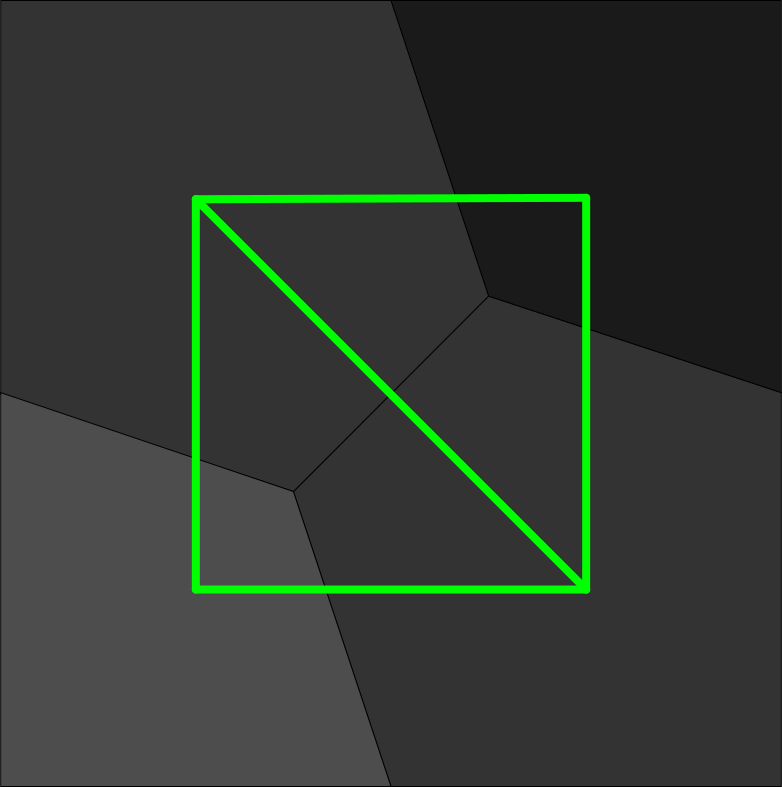
\includegraphics[width=0.8\textwidth]{assets/evil_pattern2.pdf}
  \caption{An evil pattern. A green line represents a connection (based on the
    similarity graph). The conversion to a Voronoi diagram based on the rules
    described in this document was already done in this sample.}
\end{figure}

The original Kopf-Lischinski paper describes fully connected graphs with
redundant crossing connections. The approach was to remove the redundant
crossing connections.

The existence of crossing connections prevents the conversion of the pixel graph
to Voronoi diagrams and all of them must be erased. This behaviour is kept here.

The original Kopf-Lischinski paper considers some crossing connections as
redundant, because no extra care was taken to preserve more color information,
but the \emph{evil pattern \#2} requires an extra rule to produce better
results. We handle these nodes by \textbf{NOT} removing the diagonal connection
and handling them with the heuristics for \hyperref[white_nodes]{white nodes}.

There is, however, an extra step that replaces the ``\emph{remove safe and
redundant crossing connections}'' step described in the original Kopf-Lischinski
paper. The new algorithm should detect if only one of the crossing connections
glue nodes of equal colors (as opposed to similar colors) and preserve it over
the other connection. If the detection fails, just fallback to the old
Kopf-Lischinski technique. We'll handle the new nodes using the same rules for
\hyperref[white_nodes]{white nodes}. Note that this new rule is \textbf{not} a
classic heuristic that will compete with the other heuristics (islands, sparse
pixels, \ldots{}).

This approach is an improvement, because it'll favor a pattern where cells that
share the same color will share an edge. Thus, they will be summed together in
the same polygon in later processing steps, creating splines that are more
smooth, natural and can be optimized more easily.

\subsection{The evil pattern \#3}

An example of the \emph{evil pattern \#3} follows:

\begin{figure}[H]
  \centering
  
\includegraphics[width=0.8\textwidth]{assets/evil_pattern3.pdf}
  \caption{An evil pattern. A green line represents a connection (based on the
    similarity graph). The colors of the nodes on the main diagonal are the
    same.}
\end{figure}

The \emph{evil pattern \#3} is resolved by the technique developed to handle the
\hyperref[evil_pattern2]{evil pattern \#2}. If only one of the two connections
share the \textbf{same} color, then this should be the connection preserved.

\subsection{Other evil patterns}

There are other the evil patterns (the evil pattern \#3, where the colors of the
main diagonal are different, for instance). I give up here.

The new rules are added as an extra step on the process. They are not treated
like the Kopf-Lischinski's heuristics to resolve crossing connections. I think
maybe would be possible to get some of the new rules and describe versions that
are more general and can be added to the "container" that holds the old
heuristics. To make this happen, I'd need to define the concept of "similar
color" as a set and operations on top of the set, the notion of interval and
other things and logical reasoning on top of all that. A bit of mathematical
work to improve the quality a little more, but I wanna to investigate the use of
La*b* colors (an old suggestion by Nathan) to replace the current concept of
"similar colors". I didn't replaced the current space color until now, because
YUV and La*b* behave differently and I couldn't just convert the YUV constants
that define the boundary between dissimilar colors to La*b* to achieve better
results. The current YUV constants were taken from HQx filter and I need to
define a methodology to find new constants.

The advantage of a rule that is more general and unifies behaviour is just the
beauty of a simpler rule that handles the real problem, as opposed to several
branches that are consequence of the real problem. It'd abstract the nature of
the problem better. It'd make the code simpler. It'd handle more branches. Being
a single rule that affect more branches, it'd be easier to test and better at
convincing me that the improvement is real and there will be no loss of quality
in other images.

It'd be interesting to investigate the range of voting in all heuristics and try
to come up with "fair" multipliers/strength.


\chapter{Optimizing the B-Splines}
\label{optimizing}
The vector arts generated by the previous steps are fine if you apply small
factors of zoom, but after magnifying the image several times some staircasing
artifacts become clear. To remove the staircasing artifacts, you need to
optimize the B-Spline's control points (do \textbf{not} confuse the control
points of the B-Spline with the control points of the Bézier curves, or you will
kill continuity and the result will look awful).

Kopf-Lischinski proposes the below \emph{energy} formula as the term to
optimize:

$$E^{(i)} = E^{(i)}_s + E^{(i)}_p$$

$E^{(i)}_s$ stands for smoothness energy and $E^{(i)}_p$ stands for positional
energy.

The smoothness energy formula given on the paper is:

$$E^{(i)}_s = \int\limits_{s \in r(i)} |k(s)| \mathrm{d}s$$

$k(s)$ stands for curvature at point $s$. The curvature formula for parametric
equation is given below:

$$k = \frac{x'y'' - y'x''}{(x'^2+y'^2)^{\frac{3}{2}}}$$

If you've read \href{http://pomax.github.io/bezierinfo/}{Pomax's \emph{A Primer
on Bezier Curves}}, then you already demystified the $k(s)$ formula and you are
ready to integrate it, but the Pomax's text is abstract enough for Bézier curves
of any order, then I'll help you further giving the required formulas for
quadratic Bézier curves:

$$Bezier(2, t) = (1-t)^2 w_0 + 2 (1-t) t w_1 + t^2 w_2$$

$$Bezier'(2, t) = 2 (1-t) (w_1-w_0) + 2 t (w_2-w_1)$$

$$Bezier''(2, t) = 2 (w_2 - 2 w_1 + w_0)$$

Replace the $w_i$ term by the node position on the dimension you want to
compute.

Numerical integration is easy and you can use any method you like. There is a
good text about numerical integration on
\href{http://jeremykun.com/2012/01/08/numerical-integration/}{Math $\cap$
Programming} and after you find the methods names, Wikipedia is good enough. If
you want a deep understanding on this topic, \emph{Heath's Scientific Computing}
book is a good start. You should use the $\{0..1\}$ range for the integration.

The positional energy formula is given on the paper and uses the
\href{http://en.wikipedia.org/wiki/Norm_(mathematics)}{norm} concept.


\appendix
\chapter{Complete smoothness code (without the extra color
  patch)}
\label{smoothness_code_appendix}
Originally ``published'' at \url{https://gist.github.com/vinipsmaker/6065604} on
\formatdate{23}{7}{2013}.

\lstinputlisting[language=C++]{assets/code/splines-extraction-p0.cpp}


\end{document}
